


% En-tête de l'étape : numéro bien à gauche et en haut
\noindent
\begin{minipage}[t]{0.12\textwidth}
    \vspace*{-\topskip} % Remonte le contenu au maximum
    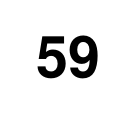
\begin{tikzpicture}
        \node[anchor=north west] at (0,0) {\usefont{OT1}{phv}{b}{n}\huge 59}; % Numéro de l'étape
    \end{tikzpicture}
\end{minipage}%
\hfill
\begin{minipage}[t]{0.7\textwidth}
    \vspace*{-\topskip}
    \section*{and voilà}
\end{minipage}%




\vspace{1em}

\begin{center}
    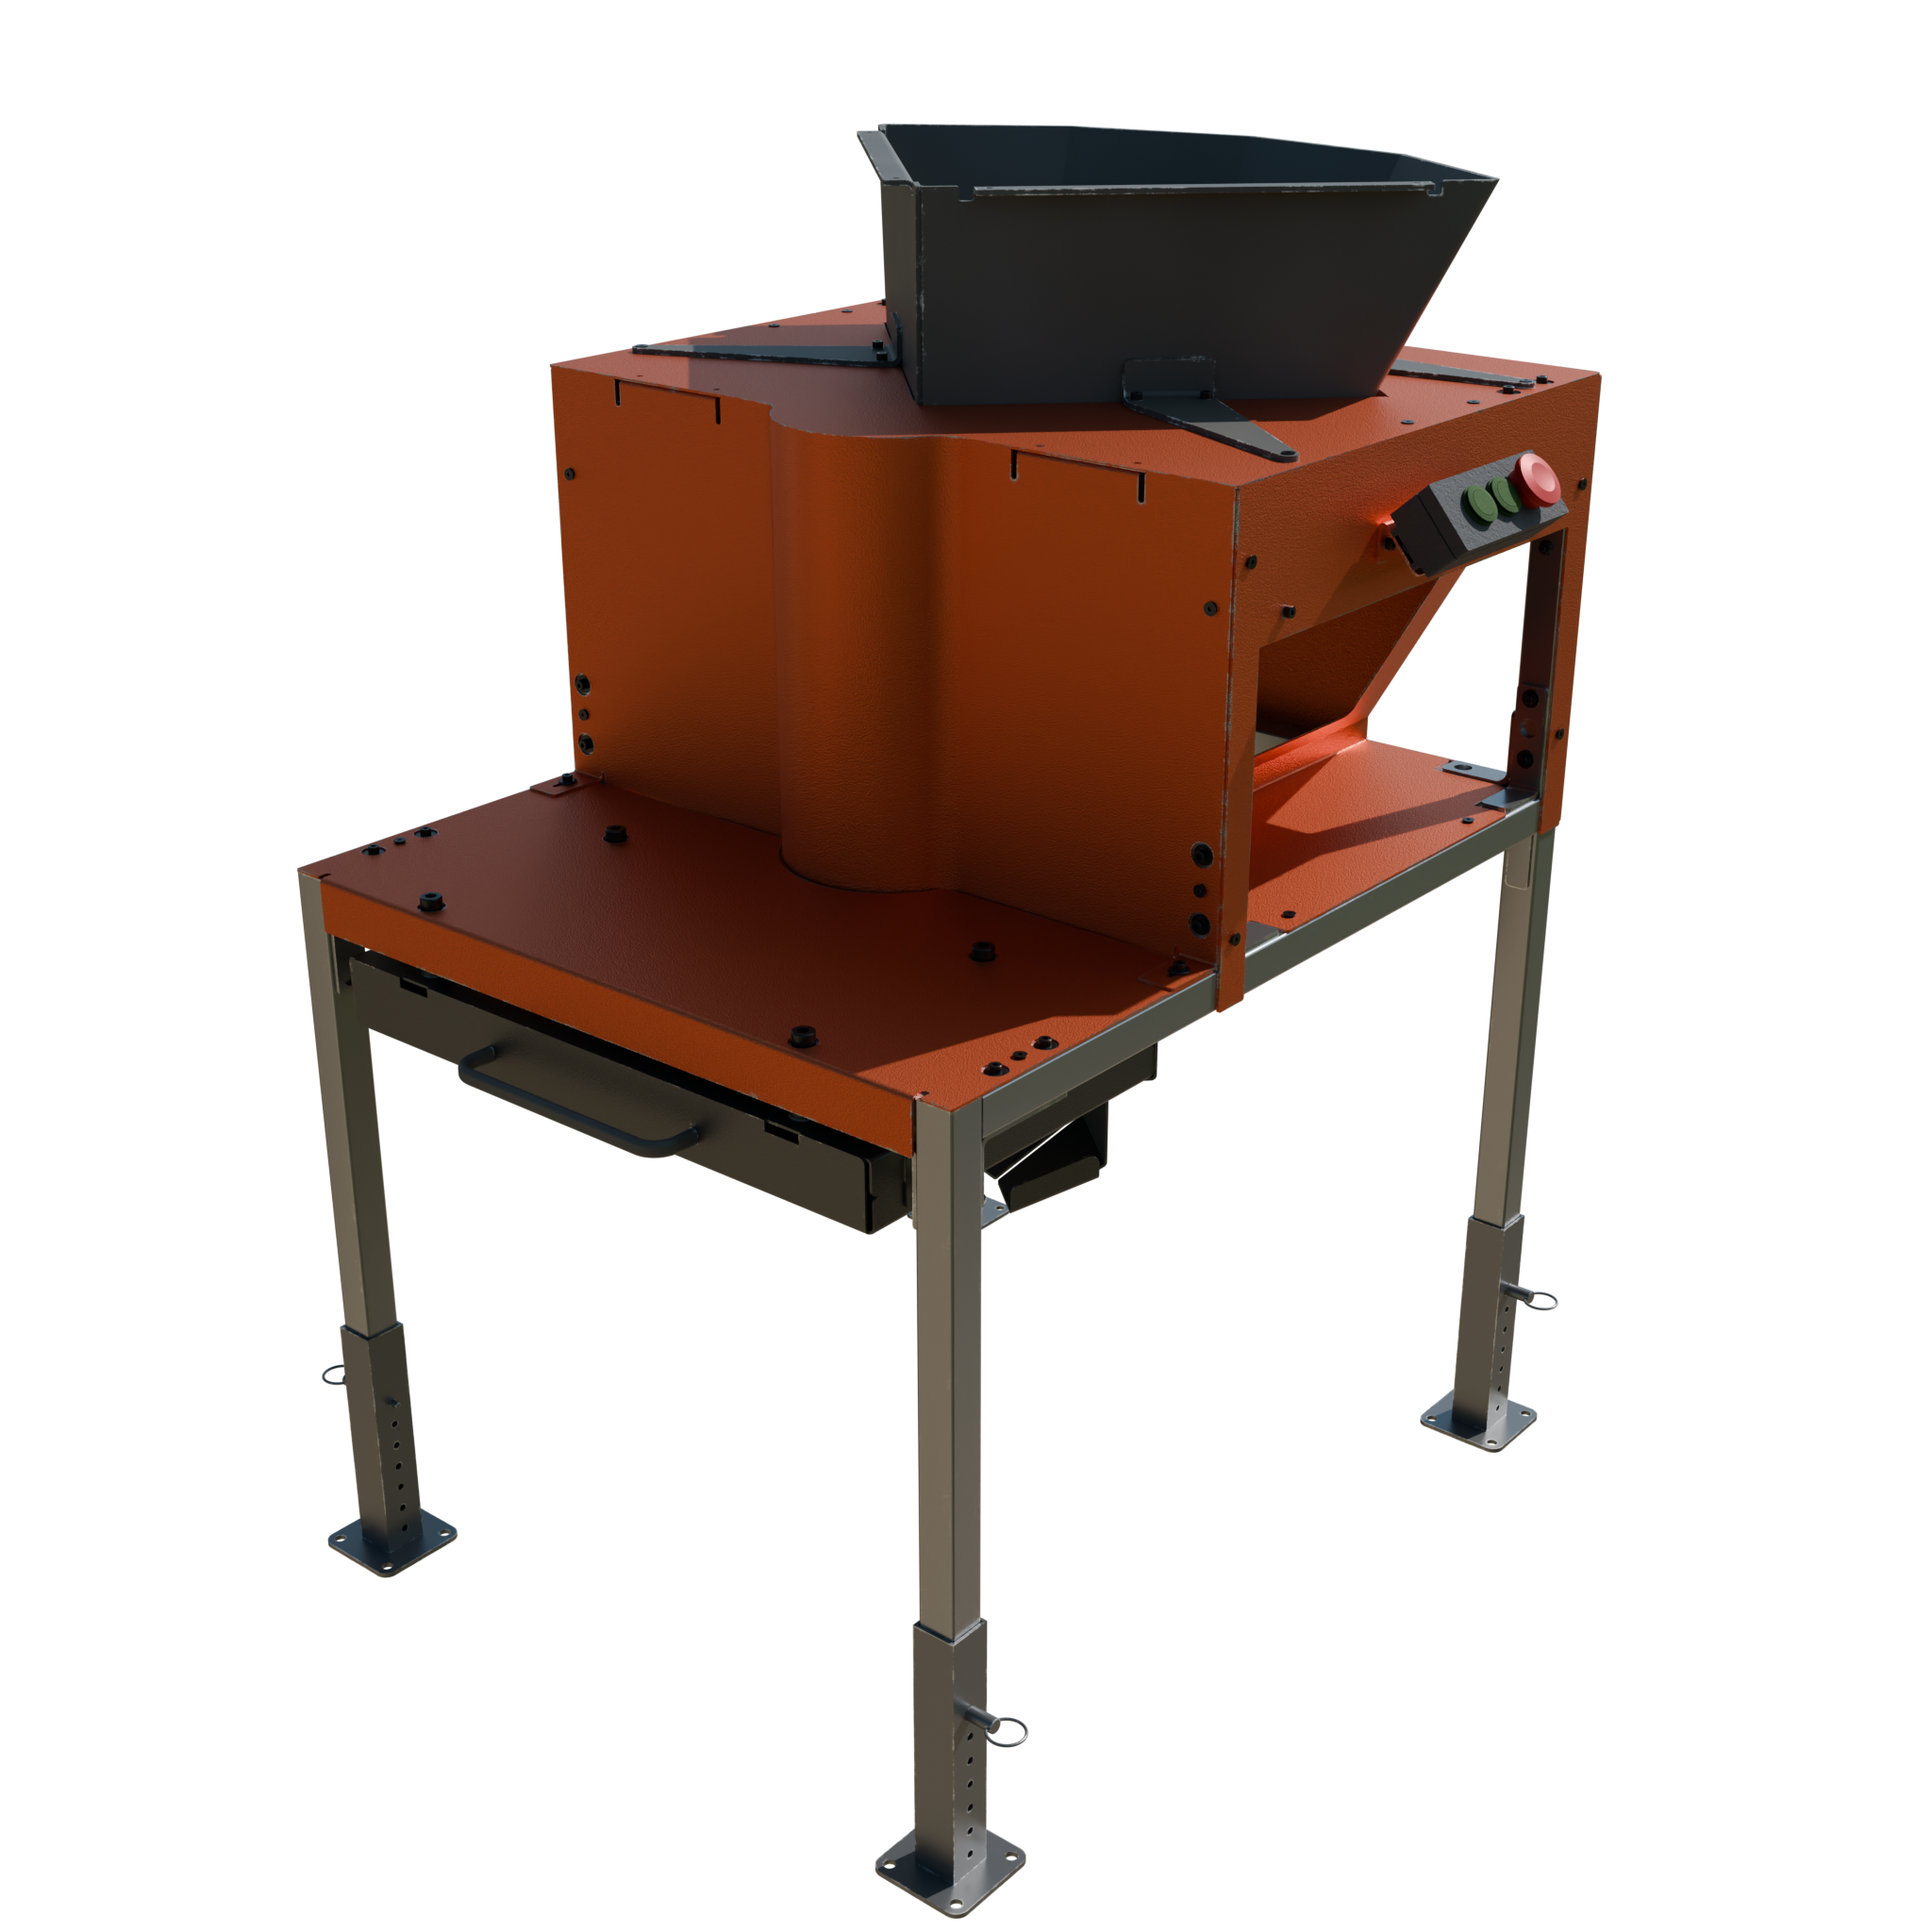
\includegraphics[height=10cm]{../images/general_vue.png}
\end{center}

\vspace{0.7em}

\begin{tcolorbox}[colback=gray!05, colframe=gray!60, boxrule=0.5pt, left=2mm, right=2mm, title=]
\textbf{Legal Notice:} This assembly manual has been designed by Rotofish Inc. All Blender renders are by W. Guilbert and the document has been generated in LaTeX by K. Renou. All its contents are the exclusive intellectual property of Rotofish Inc. Any reproduction, distribution, or unauthorized use, in whole or in part, is strictly prohibited without the express written consent of Rotofish Inc. (except for pages 42 and 69). This document is intended solely for the personal use of the original Thai purchaser. Please do not dispose of this manual in public spaces or in any manner that may contravene local environmental regulations. 
\end{tcolorbox}


